\section{Participation notes 5}
Participant: Student.

\begin{itemize}
    \item \textbf{Have them read the code-example} - Participant did not have any problem reading the code.
    \item \textbf{Have them draw the structure} - The participant started with drawing a box and called it "namespace". Within this box, two lines where written inside and was said to be the functions inside the "World" namespace. Then the participant wrote "Main" and drew two half circles on either side and said that this represented the main function. Inside of the half circles 2 lines where written as calls to the first, then second function and then a "return 0" line.
    \item \textbf{Have them submit the git URL} - URL submission went without problem and seemed to be intuitive although the participant used the cached input on the URL field and did not type it fully.
    \item \textbf{Have them get the main() implementation} - Participant was able to find implementation of main. Participant wasn't able to find the implementation of the other functions.
    \item \textbf{Participant visualization} \includepdf[pages={2}]{inc/generalAppendix/userStudies/participantsVisualization.pdf}
\end{itemize}